\section{Getting familiar with the data}

\subsection{Finding the spectral resolution}

To find the spectral resoulution of the dataset, we load the \textit{hico\_wl} array, which contains the
wavelength corresponding to band \textit{i}. We loop through the array and compare each wavelength
\textit{i} with the the previous wavelenght \textit{i-1} and we find that the average distance between
the wavelengths is $5.728 nm$, which seems to be constant between all wavelengths. 

\subsection{Relation to human color perception}

\begin{figure}
    \centering
    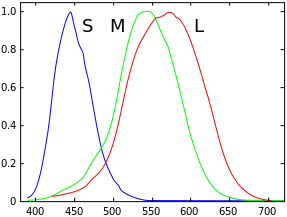
\includegraphics[width=\textwidth]{../fig/human_spectrum.png}
    \caption{Graph for the human color sensitivity curves, according to Wikipedia \cite{website:wiki_spectral}}
    \label{fig:human_spectra}
\end{figure}

The color sensitivity of the human eye is shown in \cref{fig:human_spectra}. As we can 
see, blue color has a peak around $450 nm$ (\textit{S}-curve), green peaks at $550 nm$ 
(\textit{M}-curve), and red at $600 nm$ (\textit{L}-curve). 

\subsection{Create a pseudo RGB image from the hyperspectral bands}

From the \textit{hico\_wl} array, we find that Blue (450nm) is located at index \textit{i = 8}, 
green (550nm) at \textit{i = 25}, and finally red (600nm) at \textit{i = 34}. We combine these indices from 
the HICO dataset and show it as an image to create a pseudo RGB image, shown in \cref{fig:pseudo_rgb}.


\begin{figure}
    \centering
    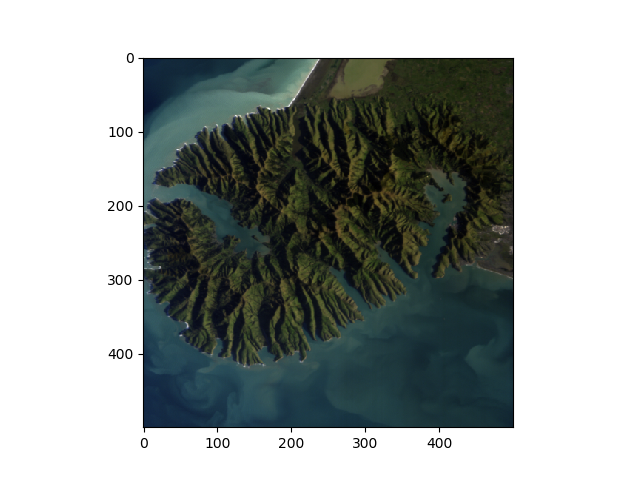
\includegraphics[width=\textwidth]{../fig/pseudo_rgb.png}
    \caption{Pseudo RGB image, showing R (600nm), G (550nm), B (450nm)}
    \label{fig:pseudo_rgb}
\end{figure}

\subsection{Representative spectra for selected points}

We want to look at the representative spectra of the points (20,20), (100,70) and (400,30).

\todo{Fix image, fix question}

\begin{figure}
    \centering
    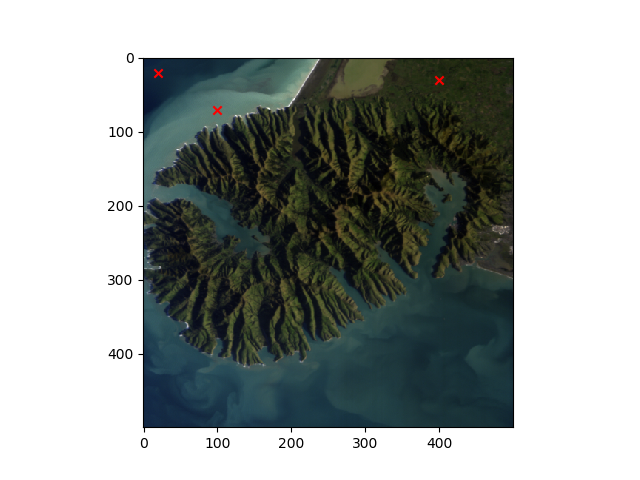
\includegraphics[width=\textwidth]{../fig/pseudo_rgb_points.png}
    \caption{Representative spectra of spesific points}
    \label{fig:point_spectra}
\end{figure}

